\chapter{The Deep Quality-Value family in Dec-POMDP}\label{ch:qvmix}
\begin{chapter_outline}

This chapter presents four value-based methods issued from the Deep Quality-Value (DQV) family for the Dec-POMDP framework.
We introduce the DQV family and detail the contribution of this chapter in Section~\ref{sec:ch4_intro}.
We then formally define DQV and the four methods in Section~\ref{sec:ch4_methods}.
The experimental setup to evaluate them is presented in Section~\ref{sec:ch4_experiments}, followed by the corresponding results in Section~\ref{sec:ch4_results}.
This chapter ends with a conclusion in Section~\ref{sec:ch4_conclusion}.

This chapter is an adapted version of the publication \citep{leroy2020qvmix} \textit{QVMix and QVMix-Max: extending the deep quality-value family of algorithms to cooperative multi-agent reinforcement learning}, P. Leroy, D. Ernst, P. Geurts, G. Louppe, J. Pisane, and M. Sabatelli. AAAI-21 Workshop on Reinforcement Learning in Games, 2021.

\end{chapter_outline}


\section{Introduction} \label{sec:ch4_intro}

This chapter introduces four methods to learn to cooperate in a Dec-POMDP, defined in Section~\ref{sec:ch3_decpomdp}.
They are adapted from the Deep Quality-Value (DQV) family of algorithm \citep{sabatelli2020deep}.
DQV methods jointly learn an approximation of the state-value function $V$ alongside an approximation of the state-action value function $Q$.
They have proven to significantly outperform popular algorithms in SARL, such as DQN and DDQN defined in Section~\ref{sec:ch2_value_based_methods}.
The four methods follow two modes of training and execution in a Dec-POMDP, introduced in Section~\ref{sec:ch3_intro}.
The methods designed for the decentralised mode are called IQV and IQV-Max.
The other two dedicated to the CTDE mode are called QVMix and QVMix-Max.
They are tested with the StarCraft Multi-Agent Challenge (SMAC) suite of environments, introduced in Section~\ref{fig:ch3_smac}.
They are compared with IQL, QMIX and MAVEN, three value-based methods in multi-agent reinforcement learning defined in Section~\ref{sec:ch3_value}.

Finally, the contributions of \citep{leroy2020qvmix} presented in this chapter can be divided into three parts.
The first is the generalisation of the DQV family of algorithms to cooperative MARL problems, their performance in the decentralised mode and their fundamental limitations.
The second is the introduction of two methods, QVMix and QVMix-Max.
Both combine the original benefits of the DQV algorithms with CTDE, resulting in a better performance than state-of-the-art techniques of their time.
The third is to link their better performance to the overestimation bias of the $Q$ function that characterises model-free RL algorithms.

\section{Methods} \label{sec:ch4_methods} 

As introduced, the work presented in this chapter revolves around the Deep Quality-Value (DQV) family of DRL algorithms \citep{sabatelli2018deepQV, sabatelli2020deep}.
These SARL techniques learn an approximation of the state value function $V$ alongside an approximation of the state-action value function $Q$.
The DQV algorithms extend the tabular RL algorithms called QV($\lambda$) learning \citep{wiering2005qv, wiering2009qv} with neural networks as function approximations.
There are two possible ways of learning a joint approximation of the $V$ function, $V(s;\phi)\approx V^{\pi^*}(s)$, and of the $Q$ function, $Q(s, u;\theta)\approx Q^{\pi^*}(s, u)$.

DQV learns an approximation of the $V$ function by minimising
\begin{equation}
    \mathcal{L}(\phi) = \mathbb{E}_{B} \bigg[\big(r_{t} + \gamma V(s_{t+1}; \phi') - V(s_{t}; \phi)\big)^{2}\bigg],
    \label{eq:ch4_dqv_v_update}
\end{equation} 
while the $Q$ function is learned by minimising 
\begin{equation}
    \mathcal{L}(\theta) = \mathbb{E}_{B} \bigg[\big(r_{t} + \gamma V(s_{t+1}; \phi')  - Q(s_{t}, u_{t}; \theta)\big)^{2}\bigg].
\label{eq:ch4_dqv_q_update}
\end{equation}
    
DQV-Max learns the $Q$ function with the same loss defined in Equation \eqref{eq:ch4_dqv_q_update} but learns the $V$ function by minimising
\begin{equation}
        \mathcal{L}(\phi) = \mathbb{E}_{B} \bigg[\big(r_{t} + \gamma \: \underset{u\in \mathcal{U}}{\max}\: Q(s_{t+1}, u; \theta') - V(s_{t}; \phi)\big)^{2}\bigg].
        \label{eq:ch4_dqv_max_v}
\end{equation}
As in DQN, the replay buffer $B$ stores transitions $\langle s_{t},u_{t},r_{t},s_{t+1}\rangle$ from which batches of transitions are sampled to update the networks.
The target network $\theta'$ and $\phi'$ are a copies of $\theta$ and $\phi$ updated periodically.

The extension to the decentralised MARL methods is straightforward, like IQL from DQN.
This leads to IQV and IQV-Max using, respectively, the DQV and DQV-Max update rules to learn $Q_a(\tau^a, u^a;\theta)$ and $V_a(\tau^a;\phi)$ independently.
For the CTDE mode, the methods are QVMix and QVMix-Max, and they follow the DQV and DQV-Max update rules to learn $Q^{mix}_{tot}(s, \mathbf{u})$.
The architecture of the $Q_a$ and the mixer network is the same as in QMIX, using the same monotonic decomposition.
In both QVMix and QVMix-Max, the $V$ network computes a central state value function $V^{mix}_{tot}(s)$ as a function of individual $V_a(\tau^a;\theta)$.
It has the same architecture as the $Q$ ones of QMIX, except they have a single output. 
The architecture is presented in Figure~\ref{fig:ch4_qvmix}.
In QVMix, $V^{mix}_{tot}$ is updated following the loss defined in Equation~\ref{eq:ch4_dqv_v_update} and with the loss defined in Equation~\ref{eq:ch4_dqv_max_v} for QVMix-Max.
Individual networks are GRU, and $B$ stores sequences of contiguous transitions instead of single transitions to train recurrent neural networks.

\begin{figure}
\centering

\begin{tikzpicture}[node distance=.5cm]

\tikzstyle{netbox} = [rectangle, rounded corners, minimum width=1cm, minimum height=1cm, draw=blue]
\tikzstyle{mixerbox} = [rectangle, rounded corners, minimum width=4.5cm, minimum height=1.5cm, draw=blue]
\tikzstyle{indixQbox} = [rectangle, rounded corners, minimum width=1.3cm, minimum height=2cm, draw=red]
\tikzstyle{io} = [minimum width=0.2cm,minimum height=0.5cm]
\tikzstyle{emptynetbox} = [rectangle, rounded corners, minimum width=1cm, minimum height=1cm]

\node (output_node) [io] {$V_{mix}^{tot}(s_t)$};
\node (mixerbox) [mixerbox, below=of output_node, yshift=-0cm, label={[xshift=-1.4cm, yshift=-1cm]$Mixer$}] {};
\node (indivQbox1) [indixQbox, below=of mixerbox, xshift=-1.2cm, yshift=-.5cm, label={[xshift=-0.22cm, yshift=.2cm]$V_{a_1}(\tau^1_t)$}] {$V_{a_1}$};
\node (indivQboxn) [indixQbox, below=of mixerbox, xshift=1.2cm, yshift=-.5cm, label={[xshift=0.22cm, yshift=.2cm]$V_{a_n}(\tau^n_t)$}] {$V_{a_n}$};
\node (mixer_net) [netbox, below=of output_node, yshift=-0.3cm] {$h_o$};
\node (param_net) [netbox, right=of mixer_net] {$h_p$};
\node (param_net2) [emptynetbox, left=of mixer_net] {};

\node (intput_node1) [io,below=of indivQbox1, yshift=-0cm, label={[xshift=1.2cm, yshift=1.2cm]. . .}] {$o^{a_1}_t$};
\node (intput_noden) [io,below=of indivQboxn, yshift=-0cm] {$o^{a_n}_t$};
\node (intput_nodestate) [io, right=of param_net] {$s_t$};
\node (intput_nodestate2) [io, left=of param_net2] {};

\draw [-Latex, thick] (intput_node1) -- (indivQbox1);
\draw [-Latex, thick] (intput_noden) -- (indivQboxn);
\draw [-Latex, thick] (indivQbox1) --  (mixer_net);
\draw [-Latex, thick] (indivQboxn) -- (mixer_net);
\draw [-Latex, thick] (param_net) -- (mixer_net) node[midway, yshift=0.3cm] {$|.|$};
\draw [-Latex, thick] (intput_nodestate) -- (param_net);
\draw [-Latex, thick] (mixer_net) -- (output_node);

%\draw[thick, rounded corners, draw=blue, fill=blue!50, opacity=0.2] ($(mixerbox.north west)+(-0.5,0.5)$) rectangle ($(indivQboxn.south east)+(1,-0.5)$);
\draw[thick, rounded corners, draw=red, fill=red!50, opacity=0.2] ($(indivQbox1.north west)$) rectangle ($(indivQbox1.south east)$);
\draw[thick, rounded corners, draw=red, fill=red!50, opacity=0.2] ($(indivQboxn.north west)$) rectangle ($(indivQboxn.south east)$);
\end{tikzpicture}
\caption{Architecture of the $V_{mix}$ network.}
\label{fig:ch4_qvmix}
\end{figure}



\section{Experiments} \label{sec:ch4_experiments}

Our experiments evaluate seven methods in total.
The four defined in this chapter, QVMix, QVMix-Max, IQV and IQV-Max and the three forming the state of the art at that time, QMIX, MAVEN and IQL, defined in Chapter~\ref{ch:cooperation}.
As a test-bed, we use SMAC and evaluate the methods on eight different maps: \texttt{3m}, \texttt{8m}, \texttt{so\_many\_baneling}, \texttt{2m\_vs\_1z}, \texttt{MMM}, \texttt{2s3z}, \texttt{3s5z} and \texttt{3s\_vs\_3z}. 
We refer the reader to Section~\ref{sec:ch3_smac} for the details on SMAC.
It is worth noting that the maps chosen for our experiments differ in complexity. 
In SMAC, the goal is to maximise the sum of discounted rewards achieved by reducing each opponent team unit's health to zero, which is called a win.

Each method is executed on every map ten times, and neural networks are trained from scratch each time.
Networks are trained for $5m$ timesteps for the first four maps mentioned above and $10m$ timesteps for the four others, chosen because of the time required to achieve convergence.
Every $20.000$ timestep, the parameters of the networks are saved to perform $24$ testing episodes.

Each algorithm uses the same hyperparameter values to compare the tested method fairly.
Specifically, we refer to the authors of QMIX, MAVEN, and IQL to determine the hyper-parameters set and keep the same values for QVMix, QVMix-Max, IQV, and IQV-Max. 
For a more thorough presentation of all used hyper-parameters, we refer the reader to the open-sourced code\footnote{\url{https://github.com/PaLeroy/QVMix}}.
As is common practice within the literature, the individual networks' parameters are shared among agents to improve the algorithms' learning speed.
This means a single individual $Q_a$ network is used for all agents.
A one-hot encoding of the agent id ($\{1,..,n\}$) is added to the observation space to allow individual networks to produce different policies per agent.

\section{Results} \label{sec:ch4_results}
We report the results of experiments in two different ways.
We start by analysing each tested method's win rate before investigating the quality of the value functions learned by all algorithms.

The means of win rate for each map and algorithm are reported in Table~\ref{tab:main_results}. 
Suppose the algorithms perform equally in terms of overall performance, meaning the average win rate is the same. 
In that case, we consider the one which significantly converges the fastest to be the best-performing algorithm.
Please note that reporting an episode's win rate is a good indicator of the quality of an agent's learned policy since, as introduced in the previous section, a win directly corresponds to the best achievable sum of rewards an agent can receive.

\begin{table*}
    \centering
    \caption{
    Means of win rates achieved in eight scenarios at the end of training by QMIX, MAVEN, QVMix, QVMix-Max, IQL, IQV, and IQVMax. 
    In the first four scenarios, \texttt{3m}, \texttt{8m}, \texttt{so\_many\_baneling} and \texttt{2m\_vs\_1z}, it is measured after $5$ millions training timesteps.
    In the last four, \texttt{MMM}, \texttt{2s3z}, \texttt{3s5z} and \texttt{3s\_vs\_3z} it is measured after $10$ millions training timesteps.
    We report the best and second-best means by \textbf{bolding} and \underline{underlining} them. When results are equivalent, the cells report the fastest and second-fastest method that reaches a win rate of $100\%$ as shown in Figure~\ref{fig:all_win_curves}.}
    \setlength\tabcolsep{4.5pt}
\begin{tabular}{cccccccc}
        \toprule
        
        Map & QMIX & MAVEN &     QVMix & QVMix-Max  & IQL & IQV & IQV-Max\\
        \midrule
         \texttt{3m} & \underline{100} & 98.7 &   \textbf{100} & 100 & 93.3 & 93.3& 96.6 \\
        %\hline
        
         \texttt{8m} & 96.6& \underline{98.3} &  \textbf{100} & 96.6 & 83.3& 93.3& 90\\
        %\hline
        
         \texttt{so\_many\_baneling} & \underline{100} & 97  & \textbf{100}& 100& 50 & 40 & 40\\
        %\hline
        
        \texttt{2m\_vs\_1z} & \underline{100} & 100 &\textbf{100} & 96.6  & 100 & 100 & 100\\
        \midrule
        
       \texttt{MMM} & \textbf{100} & \underline{97.0} & 93.3 & 96.6  & 61.6 & 83.3 & 50 \\
        %\hline
        
        \texttt{2s3z}  & 96.6 & \underline{97.5} &  96.6 & \textbf{100} & 59.9 & 56.6 & 40 \\
        %\hline
        
        \texttt{3s5z} & 40 & 40.8 &\textbf{86.6} & \underline{43.3}  & 16.6 & 13.3 & 0 \\
        %\hline
        
        \texttt{3s\_vs\_3z}  & \underline{100} & 97.9  &  \textbf{100} & 100  & 83.3 & 76.6 & 63.3 \\
        \bottomrule
    \end{tabular}
    
% \begin{subtable}{\linewidth}
% \centering
% \begin{tabular}{|c|c|c|c|c||c|c|c|}
%         \hline
%         Map & QMIX & MAVEN &     QVMix & QVMix-Max  & IQL & IQV & IQV-Max\\
%         \hline
%         \texttt{3m} & \underline{}100 & 98.7 &   bf100 & 100 & 93.3 & 93.3& 96.6 \\
%         %\hline
        
%          \texttt{8m} & 96.6& \underline{}98.3 &  bf100 & 96.6 & 83.3& 93.3& 90\\
%         %\hline
        
%          \texttt{so\_many\_baneling} & \underline{}100 & 97  & bf100& 100& 50 & 40 & 40\\
%         %\hline
        
%          \texttt{2m\_vs\_1z} & \underline{}100 & 100 &bf100 & 96.6  & 100 & 100 & 100\\
%         \hline
% \end{tabular}
% \subcaption[]{5m training timesteps.}
% \end{subtable}%

% \begin{subtable}{1\linewidth}
% \centering
% \begin{tabular}{|c|c|c|c|c||c|c|c|}
%         \hline
%         Map & QMIX & MAVEN &     QVMix & QVMix-Max  & IQL & IQV & IQV-Max\\
        
%             \hline
%        \texttt{MMM} & bf100 & \underline{}97.0 & 93.3 & 96.6  & 61.6 & 83.3 & 50 \\
%         %\hline
        
%         \texttt{2s3z}  & 96.6 & \underline{}97.5 &  96.6 & bf100 & 59.9 & 56.6 & 40 \\
%         %\hline
        
%         \texttt{3s5z} & 40 & 40.8 &bf86.6 & \underline{}43.3  & 16.6 & 13.3 & 0 \\
%         %\hline
        
%         \texttt{3s\_vs\_3z}  & \underline{}100 & 97.9  &  bf100 & 100  & 83.3 & 76.6 & 63.3 \\
%         \hline
% \end{tabular}
% \subcaption[]{10m training timesteps.}
% \end{subtable}


    \label{tab:main_results}
\end{table*}

We start by observing the differences in performance between the decentralised mode methods IQL, IQV, and IQV-Max and their respective CTDE extensions QMIX, QVMix, QVMix-Max, and MAVEN.
As one might expect, we can see from the results reported in Figure~\ref{fig:ch4_2m1zwin} that methods for the decentralised mode converge slowly when compared to their CTDE counterparts on the considered \texttt{2\_vs\_1z} map.
This is particularly interesting since it shows that the DQV family of algorithms can be successfully adapted to MARL, both in the decentralised mode and the CTDE one.
However, these results are challenged once the number of agents in the maps increases: examples of such maps are \texttt{so\_many\_baneling}, \texttt{MMM} or \texttt{3s5z}.
The performance of decentralised methods starts to drop, highlighting that CTDE methods learn faster once the complexity of the training scenario increases, as is reported both in Table~\ref{tab:main_results} and Figure~\ref{fig:all_win_curves}, where the evolution of the win rate of each algorithm on every tested map is presented.
These win rate curves provide the variance between training executions.
It is essential to highlight that all methods suffer from a significant variance.
However, it is difficult to conclude which one suffers the most.

\begin{figure}
\centering
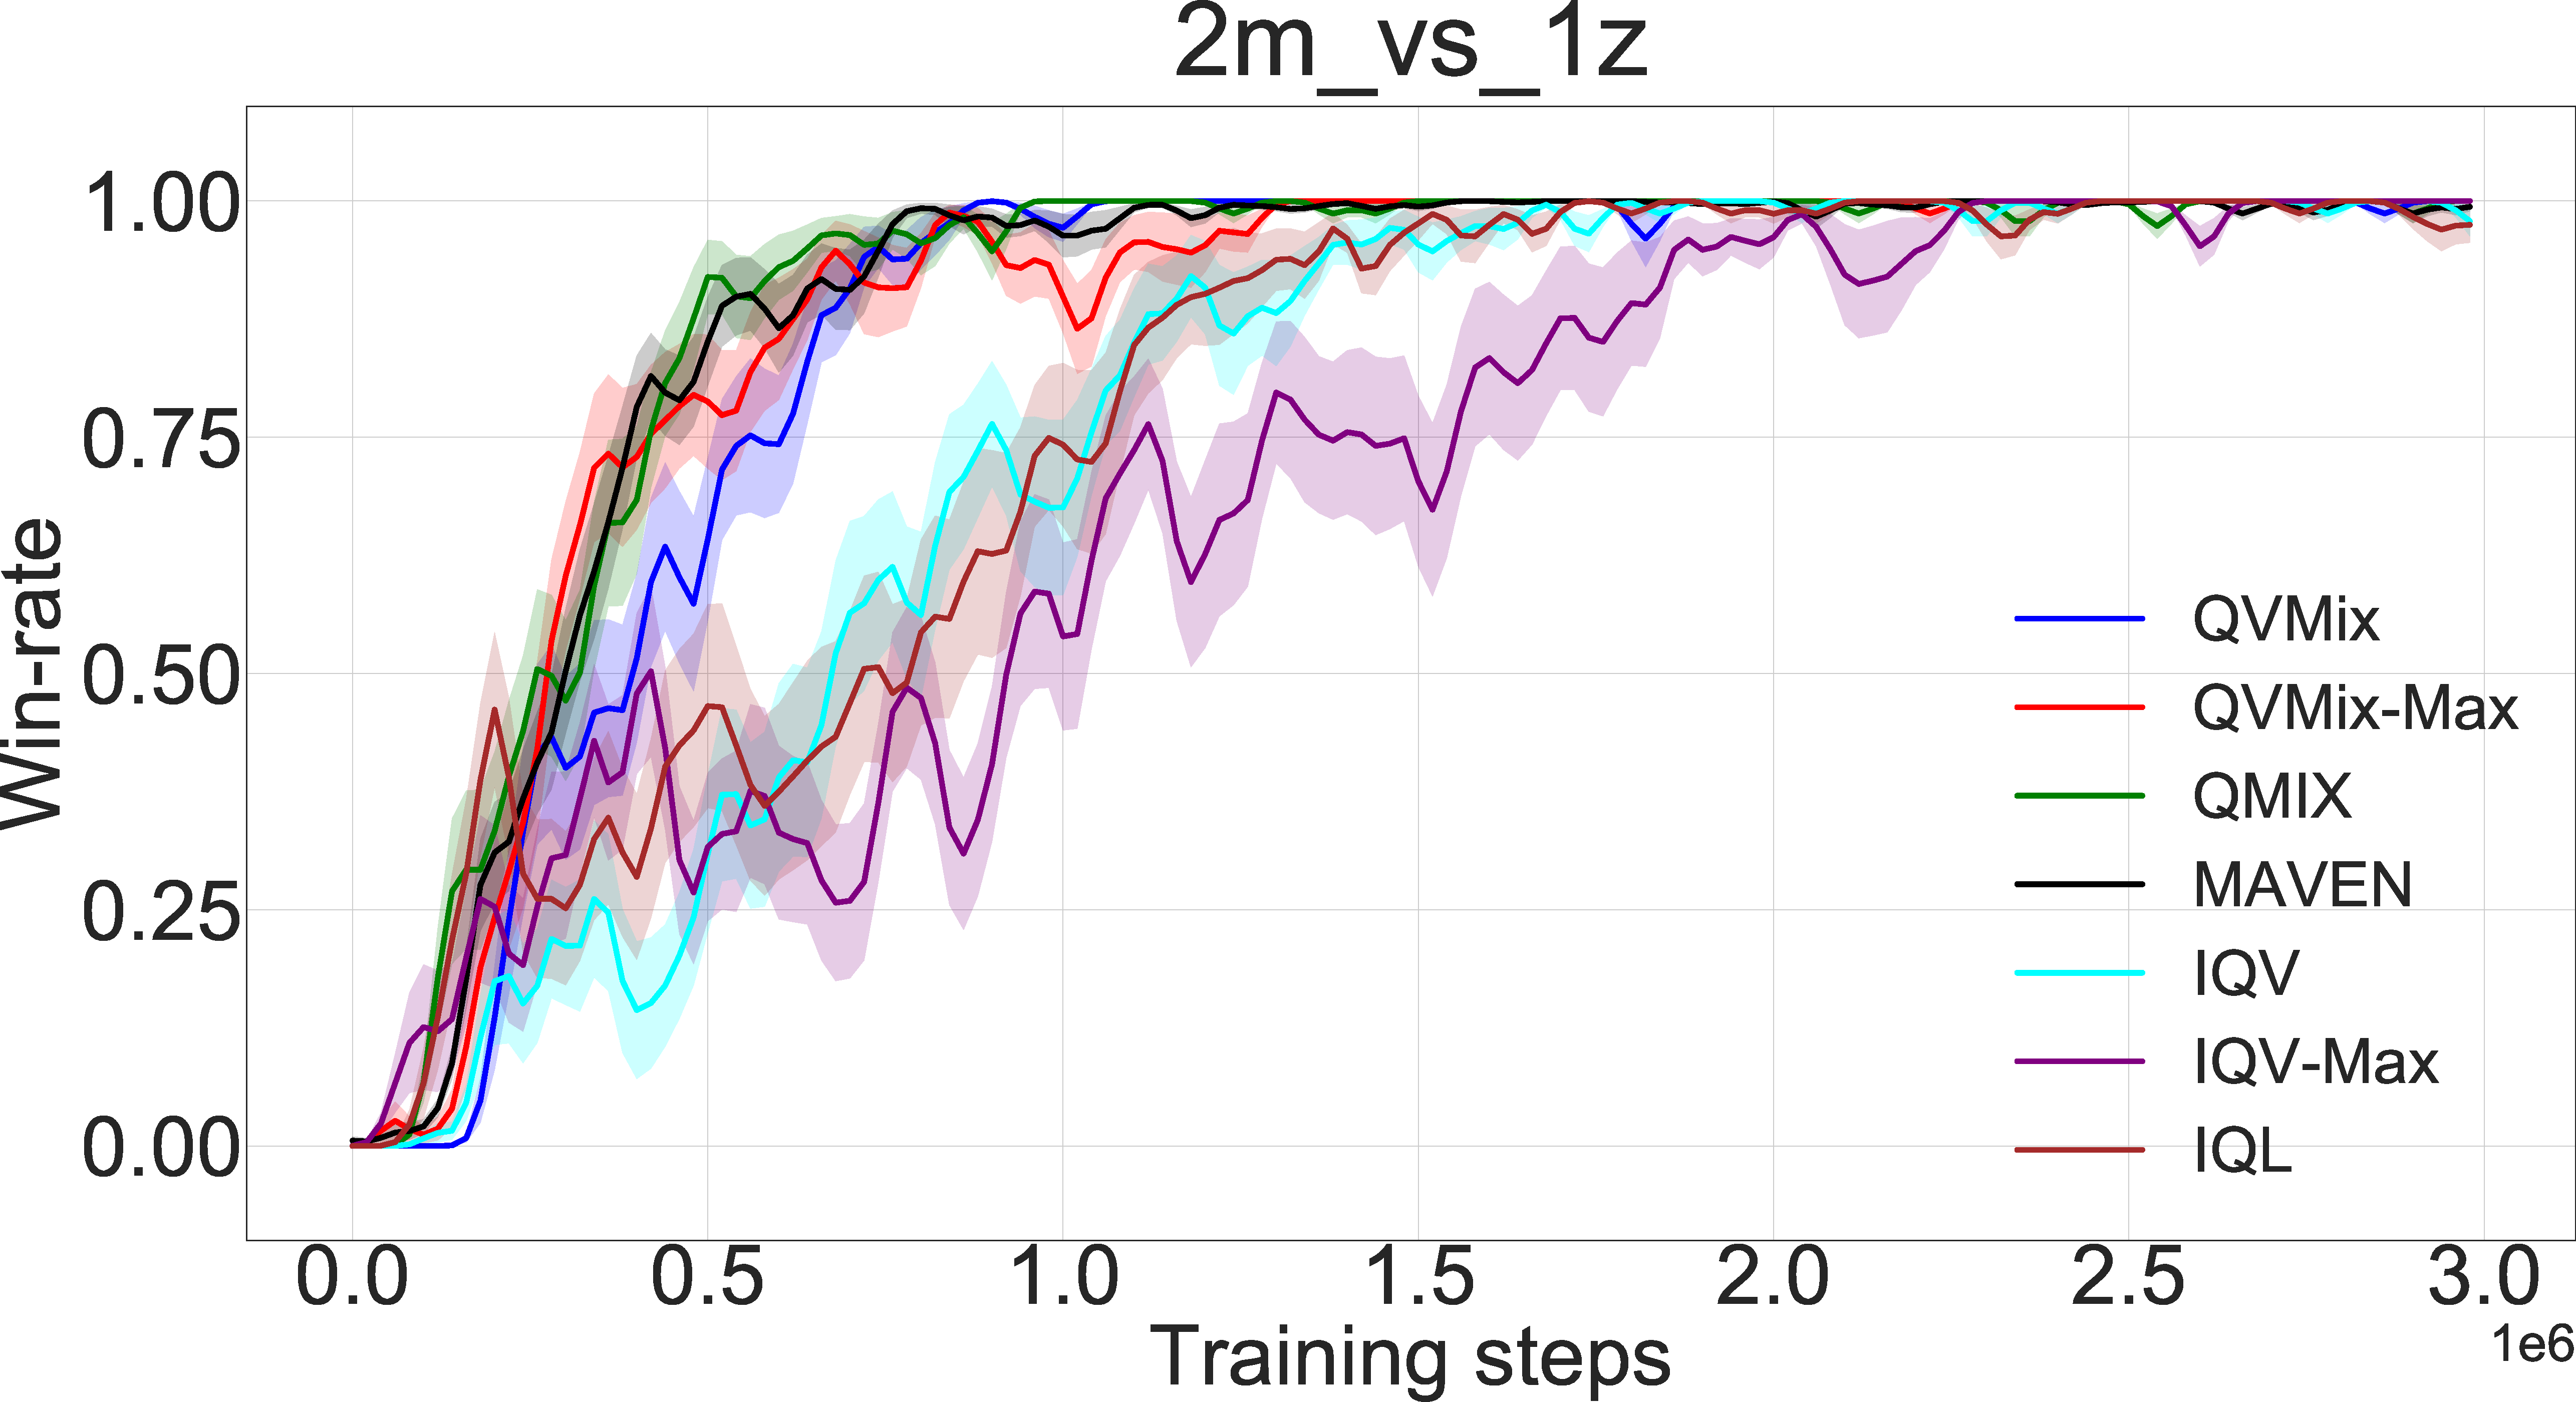
\includegraphics[width=.8\linewidth]{tex_thesis/figures/ch4/2m1zall.pdf}
\caption{Mean of win rates achieved in the \texttt{2m\_vs\_1z} map by QVMix, QVMix-Max, QMIX, MAVEN, IQV, IQVMax and IQL. The error band is proportional to the variance of the measure. We observe that all CTDE methods result in faster training than decentralised ones. All four novel algorithms based on the DQV algorithms can be successfully used in cooperative MARL.}
\label{fig:ch4_2m1zwin}
\end{figure}

\begin{figure*}
\centering
\includegraphics[width=.95\linewidth]{tex_thesis/figures/ch4/all_win.pdf}
\caption{Means of win rates achieved by QVMix, QVMix-Max, QMIX, MAVEN, IQV, IQVMax and IQL in eight scenarios. Top to bottom, left to right, the scenarios are \texttt{3m}, \texttt{8m}, \texttt{so\_many\_baneling}, \texttt{2m\_vs\_1z}, \texttt{MMM}, \texttt{2s3z}, \texttt{3s5z} and \texttt{3s\_vs\_3z}. The error band is proportional to the variance of win rates.}
\label{fig:all_win_curves}
\end{figure*}

Therefore, directing attention to CTDE methods, we observe that only QVMix and QVMix-Max perform as well as QMIX and MAVEN in most of the eight maps.
When we consider the \texttt{MMM}, \texttt{3m}, \texttt{2m\_vs\_1z} and the \texttt{so\_many\_baneling} maps, we observe that there is no significant difference between the performance that is obtained by our algorithms and that of QMIX and MAVEN. 
All methods converge towards the best possible winning rate and, in terms of convergence speed, perform closely.

However, when considering the \texttt{2s3z}, \texttt{3s5z} and \texttt{8m} maps, we observe that the performance of QVMix results in even faster learning. 
Of greater interest, when looking at the results obtained on the \texttt{3s5z} map, QVMix is the only algorithm approaching the best possible win rate.
It is also worth noting that QVMix-Max's performance is always competitive with that of QVMix, QMIX, and MAVEN.
These results are unsurprising since a similar performance was observed when DQV-Max was tested in a SARL setup by \cite{sabatelli2020deep}.

\begin{figure*}
\centering
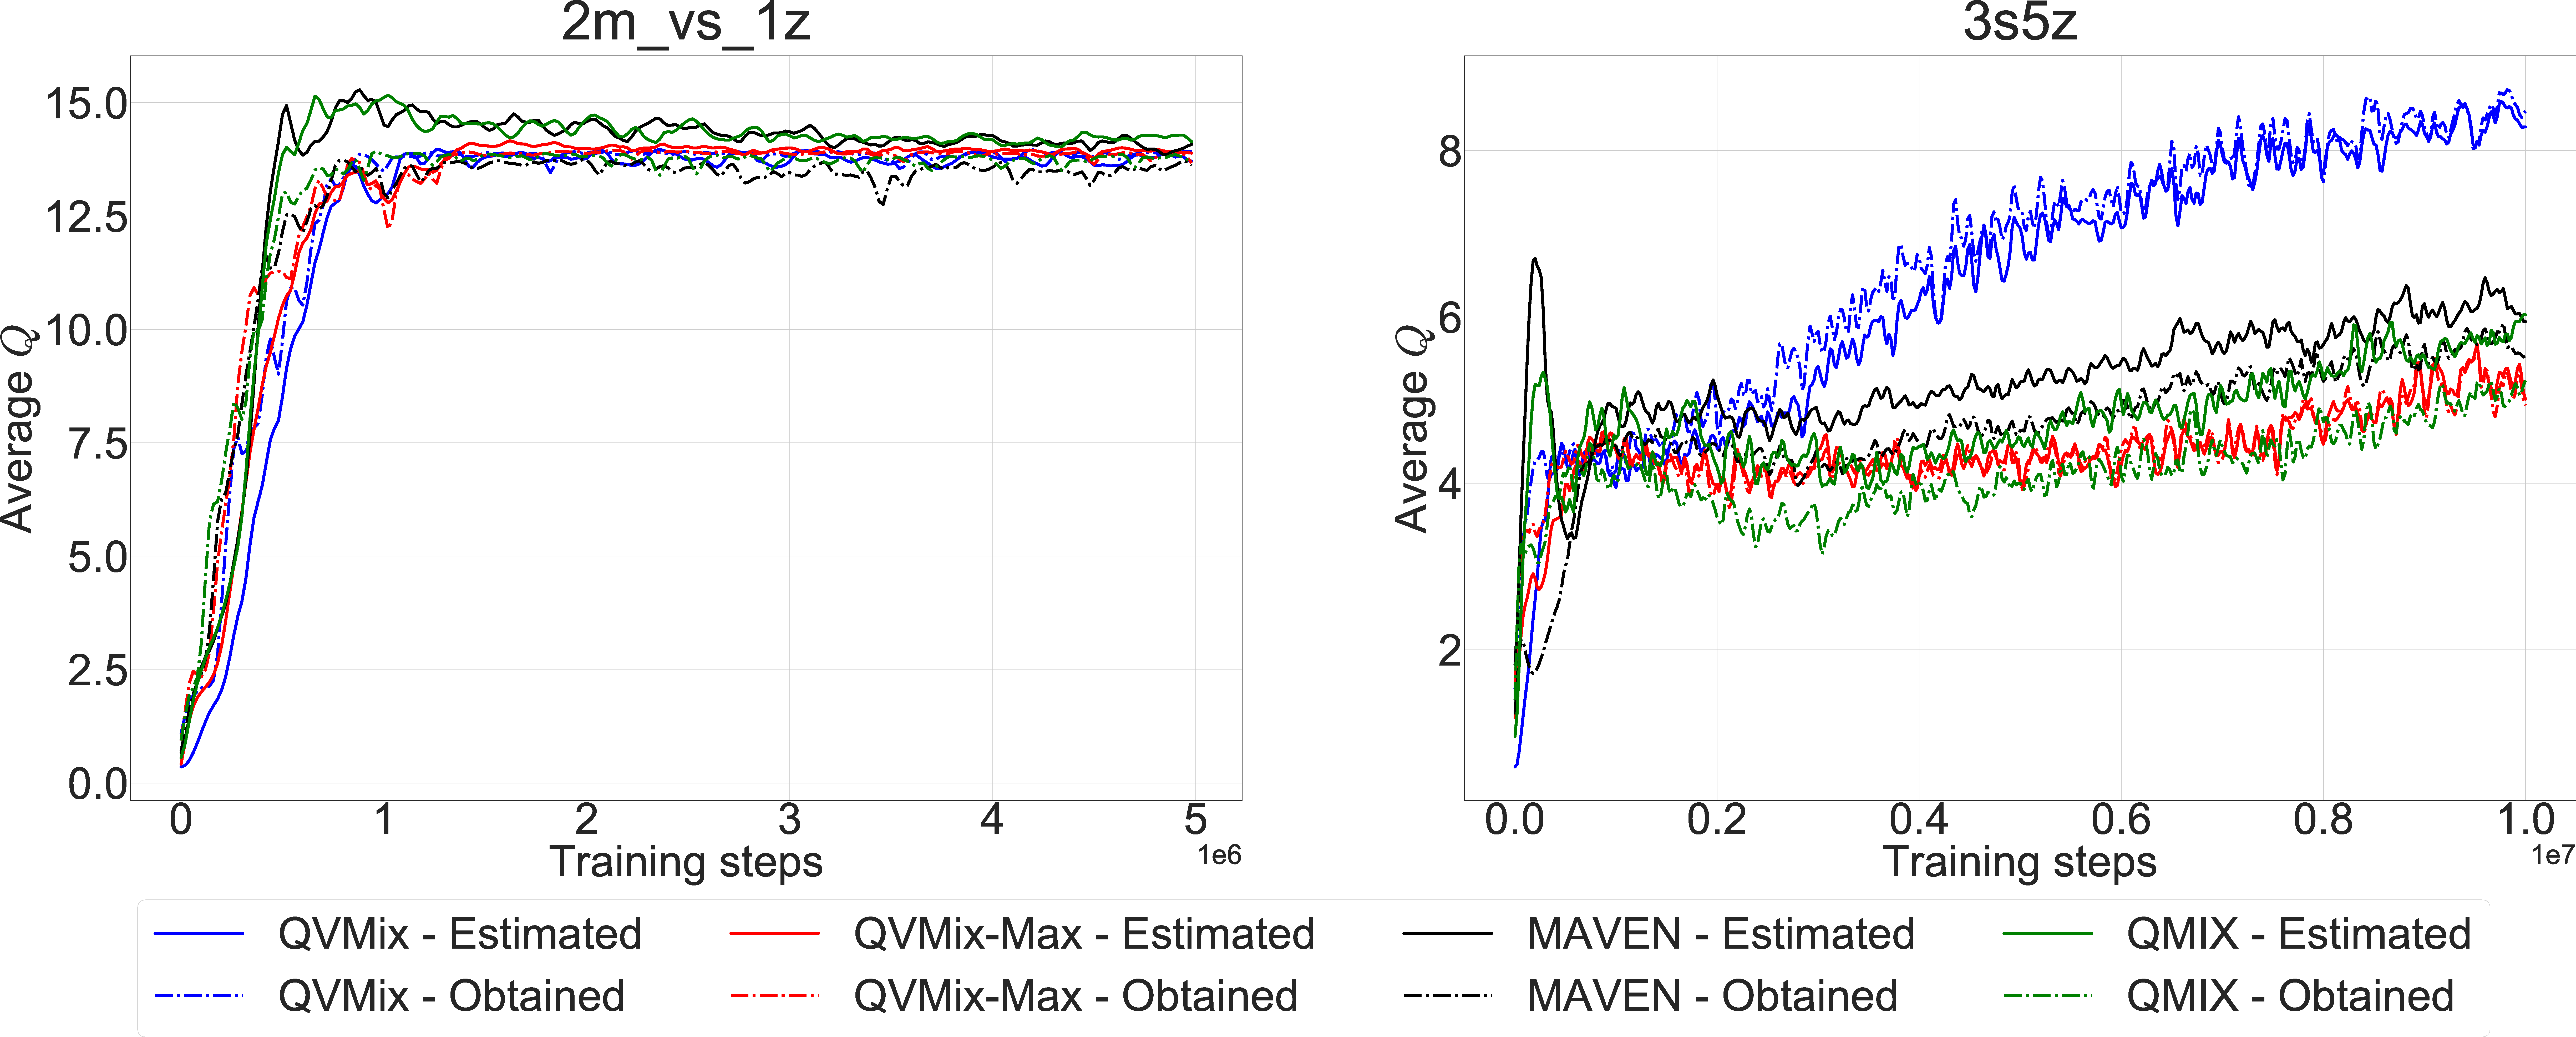
\includegraphics[width=.95\linewidth]{tex_thesis/figures/ch4/2m1z3s5zQ.pdf}
\caption{$Q$ values obtained and estimated when training QVMix, QVMix-Max, MAVEN and QMIX. Dash-dotted lines represent the obtained $Q$ values, while solid lines represent the estimated ones.}
\label{fig:exp_plots_overestim:q_best_worse}
\end{figure*}

To understand the reasons behind why QVMix is the best performing algorithm overall, we analyse how well each method estimates the state-joint-action value function $Q_{mix}^{tot}(s_t, \mathbf{u_t})$. 
Since, in most maps, decentralised methods do not perform as well as CTDE methods, we restrict our analysis to CTDE algorithms only where their respective mixer networks give the estimated $Q(s_t, \mathbf{u_t})$.
Since the state space of the maps provided by the SMAC environment is not finite, it is not impossible to compute the exact $Q_{tot}(s_t, \mathbf{u_t})$ for all states to compare them with the estimations.
To overcome this problem, we compute the discounted sum of rewards obtained with the current policy in each visited state during an episode and compare the results with the value function inferred from the $Q_{tot}$ values estimated by the mixer network for these states.
The closer the estimates are to the actual $Q(s_t, \argmax_{\mathbf{u}}(Q(s_t,\mathbf{u})))$, the more accurate the learned value function is.

For this experiment, we selected two different maps: the \texttt{2m\_vs\_1z} map, which corresponds to the map on which the best results have been achieved by all methods at the same time, and the \texttt{3s5z} map, which on the other hand, is the map on which QVMix, and others, performed less well.
In Figure~\ref{fig:exp_plots_overestim:q_best_worse}, we report the averaged estimated $Q$ values, represented by the solid lines, and the actual discounted sum of rewards, represented by the dash-dotted lines.
All are computed for each visited state at testing time.
In both scenarios, we can observe that the $Q$ values estimated by QMIX and MAVEN suffer from the overestimation bias of the $Q$ function, while this is not the case for QVMix and QVMix-Max.
Therefore, we justify the better quality of QVMix and QVMix-Max policies by better approximating the $Q$ functions.
However, further work is required to understand this phenomenon in more detail.

\section{Discussion and future work} \label{sec:ch4_conclusion}

In this chapter, we introduced four new value-based methods for training a team of agents in a Dec-POMDP.
Two of our methods, IQV and IQVMax, are designed for the decentralised mode, while the two dedicated to the CTDE mode are QVMix and QVMix-Max.
We compared these algorithms with three methods from the literature, using the StarCraft Multi-Agent Challenge as a benchmark.
We have shown that QVMix and QVMix-Max achieve the same results as popular techniques QMIX and MAVEN and that QVMix can result in faster and better learning in some maps.
We suggest that this better performance can be related to the fact that QVMix seems to suffer less from the overestimation bias of the $Q$ function.

In future work, it would be interesting to analyse each agent's behaviour and study the impact of the value function in the optimisation procedure.
Furthermore, following the recommendations from \citep{gorsane2022towards}, testing in different environment suites is crucial. 
The next chapter also tests QVMix, which provides performance similar to QMIX, as is the case with SMAC.
In this following study, QVMix is also compared to policy-based methods, which are missing in the analysis of this chapter and are justified by the performance of existing ones at the time of development.
The number of agents is also limited in SMAC.
The next chapter covers setting up to 100 agents, which allows testing the scalability of methods.

In Chapter \ref{ch:cooperation}, we defined the dueling structure, which is sometimes considered close to the DQV family because both approximate the state value function $V$ to obtain the $Q$.
We hereafter explain how different they are.
In DQV methods, the $V$ network approximates the expected return of the optimal policy $\approx V^{\pi^*}(s)$ to provide a target to train a $Q$ network.
Conversely, in the dueling structure $Q=V+A$, the $V$ network does not play the target role in the loss but allows $Q$ to be decomposed.
Nevertheless, QPLEX and QVMix performance are compared in the next chapter.
Finally, LAN proposes to learn a single central $V$ and independent advantage $A$ to compute independent $Q_a$ using the dueling structure.
It would be interesting to study how to relax the constraint of the $Q$ mixer in QVMix and QVMix-Max to train only independent $Q_a$, using a single central $V$ approximation as a target.


\todo{read Matthia's thesis to add more?}
\todo{std fraction}